\subsubsection*{الف}
این دستور Type I و از نوع Branch است. برای اضافه کردن این دستور به معماری خود، کافیست ALUOp آن را با دستور Branch برابر قرار دهیم و مقدار Funct های آن‌ها را متفاوت در نظر بگیریم.
\subsubsection*{ب}
جداول و معماری فوق به این صورت تغییر خواهند کرد:
\setLTR

$\qquad\quad\quad\quad\quad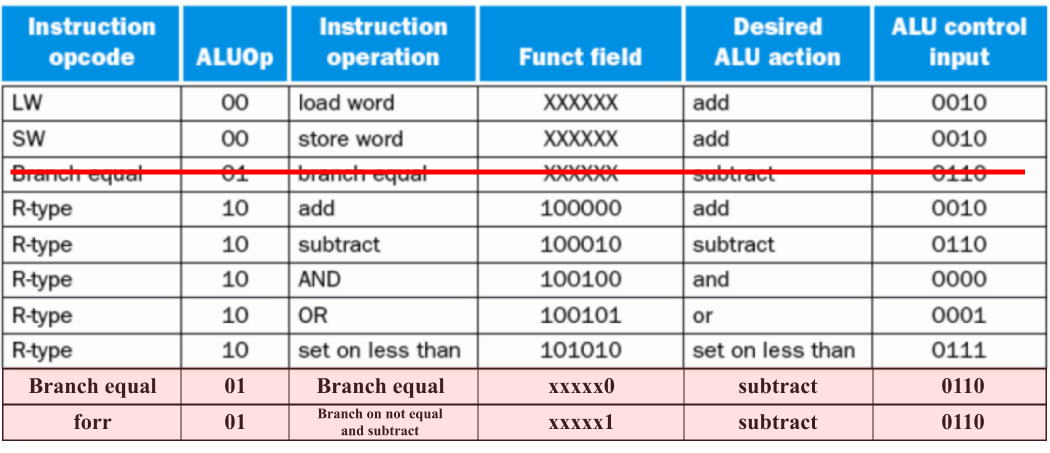
\includegraphics[width=0.7\linewidth]{figs/8.png}$

\setRTL

\setLTR

$\qquad\quad\quad\quad\quad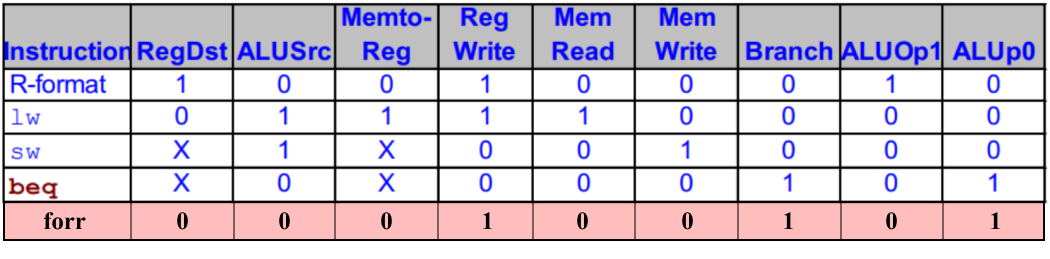
\includegraphics[width=0.7\linewidth]{figs/9.png}$ 

\setRTL 

\setLTR

$\quad\qquad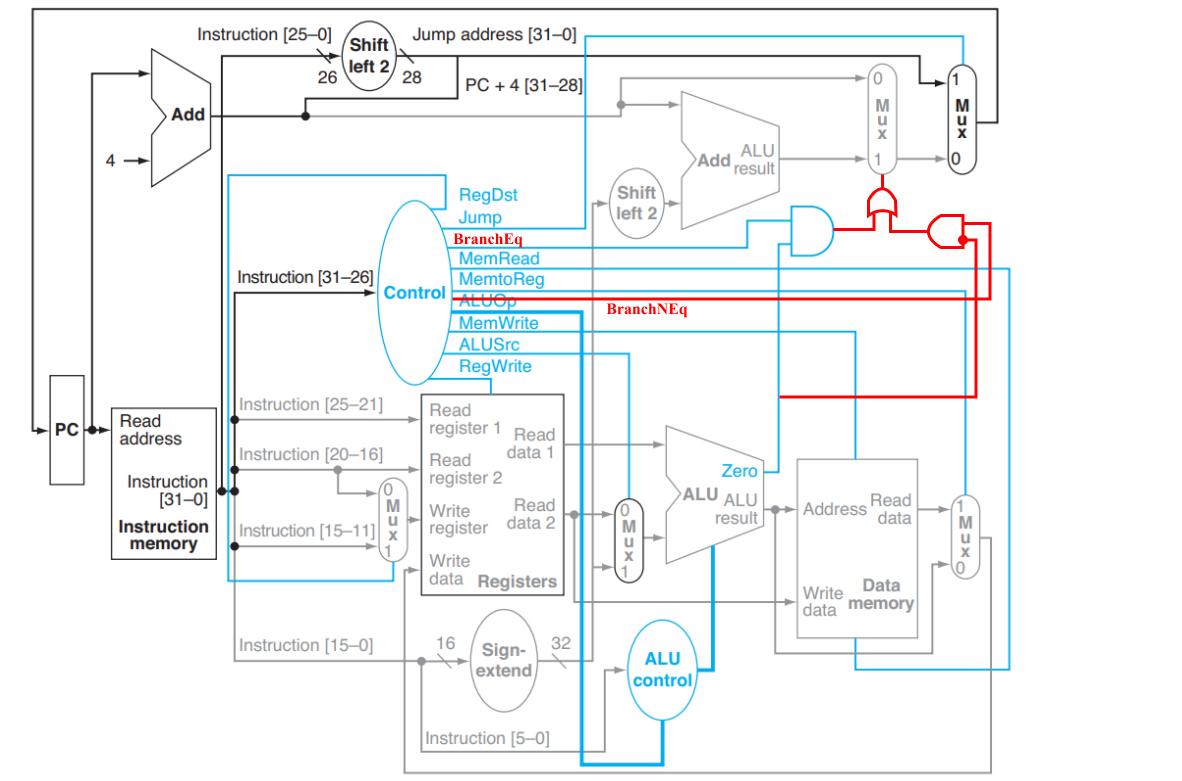
\includegraphics[width=1\linewidth]{figs/10.png}$

\setRTL